\documentclass[conference]{IEEEtran}

\usepackage{cite}
\usepackage{amsmath,amssymb}
\usepackage{booktabs}
\usepackage{graphicx}
\usepackage{placeins}
\usepackage{float}
\usepackage{array}
\usepackage{url}

\graphicspath{{figures/}}
\DeclareGraphicsExtensions{.pdf,.png}
\setlength{\textfloatsep}{5pt plus 2pt minus 2pt}
\setlength{\dbltextfloatsep}{5pt plus 2pt minus 2pt}
\setlength{\floatsep}{4pt plus 1pt minus 1pt}
\setlength{\abovecaptionskip}{3pt}
\setlength{\belowcaptionskip}{0pt}

\title{AERIS: Boundary-Mapped Reliable Routing for Wireless Sensor Networks under Heterogeneous Channels}

\author{
\IEEEauthorblockN{Anonymous Author(s)}
\IEEEauthorblockA{Submission for IEEE LCN 2026 (double-blind review)}
}

\begin{document}

\maketitle

\begin{abstract}
Reliable routing remains a challenging problem in wireless sensor networks under heterogeneous and unstable channel conditions. Existing WSN protocols address this challenge through clustering, chain-based aggregation, threshold-triggered reporting, or collection-tree parent selection. However, classical protocols often suffer from fragile long-range uplinks, while advanced collection-tree designs introduce complex control logic, leaving room for a simple and auditable reliability-first solution. To address these limitations, an adaptive environment-aware routing protocol, AERIS, is proposed. A context-adaptive intra-cluster forwarding mechanism selects direct, chain, or two-hop transmission based on local channel quality, residual energy, and node utilization. A Gateway-assisted uplink mechanism reinforces the fragile cluster-head-to-base-station path. Additionally, a sparse Skeleton reserve backbone serves as a deterministic fallback. Experimental results demonstrate that AERIS ranks first in 21 of 28 evaluation cells and top-two across all 28 cells compared to classical WSN baselines. In a fixed 100-node evaluation, AERIS improves PDR by 30.1, 24.2, 26.0, and 41.4 percentage points over PEGASIS, TEEN, HEED, and LEACH, respectively.
\end{abstract}

\begin{IEEEkeywords}
wireless sensor networks, reliable routing, cross-platform evaluation, deployment boundary
\end{IEEEkeywords}

\section{Introduction}
Wireless sensor network (WSN) routing is traditionally evaluated through the lens of energy efficiency, yet in practical deployments, link stability often dictates the fundamental usability of a routing rule~\cite{akyildiz2002survey,rault2014energy,kandris2009power}. Classical protocols address this trade-off via distinct architectural priorities: LEACH focuses on clustered forwarding~\cite{heinzelman2000energy}, PEGASIS employs chain-based aggregation~\cite{lindsey2002pegasis}, HEED incorporates residual-energy-aware head election~\cite{younis2004heed}, and TEEN restricts reporting to event-triggered thresholds~\cite{manjeshwar2001teen}. In real-world scenarios, the problem is compounded because low-power WSN channels are inherently asymmetric, environment-sensitive, and prone to instability near connectivity thresholds~\cite{zuniga2004analyzing,zamalloa2007analysis,baccour2012radio}.

The practical challenge is not to identify a single dominant routing family. It is to find the regimes where a simple, auditable controller outperforms classical energy-first designs, and the regimes where richer collection-tree or RPL-style stacks should remain the default. AERIS addresses that question with fixed-rule control rather than learned heuristics. Its architecture combines Context-Adaptive Switching (CAS) for intra-cluster mode selection, Gateway reinforcement for CH-to-BS uplinks, and a sparse Skeleton reserve backbone.

We make three primary contributions:
\begin{enumerate}
    \item We present AERIS as a fixed-rule routing design whose online decisions are traceable to channel and topology inputs.
    \item We evaluate it with a five-protocol NS-3 comparison and a seven-protocol boundary sweep, including simplified CTP/RPL-MRHOF baselines and a collision-aware stress layer, while keeping ranking evidence separate from stress evidence.
    \item Through ablation and pooled trade-off statistics, we show that the main reliability gain comes from Gateway support and is accompanied by earlier node death.
\end{enumerate}

\begin{figure*}[t]
\centering
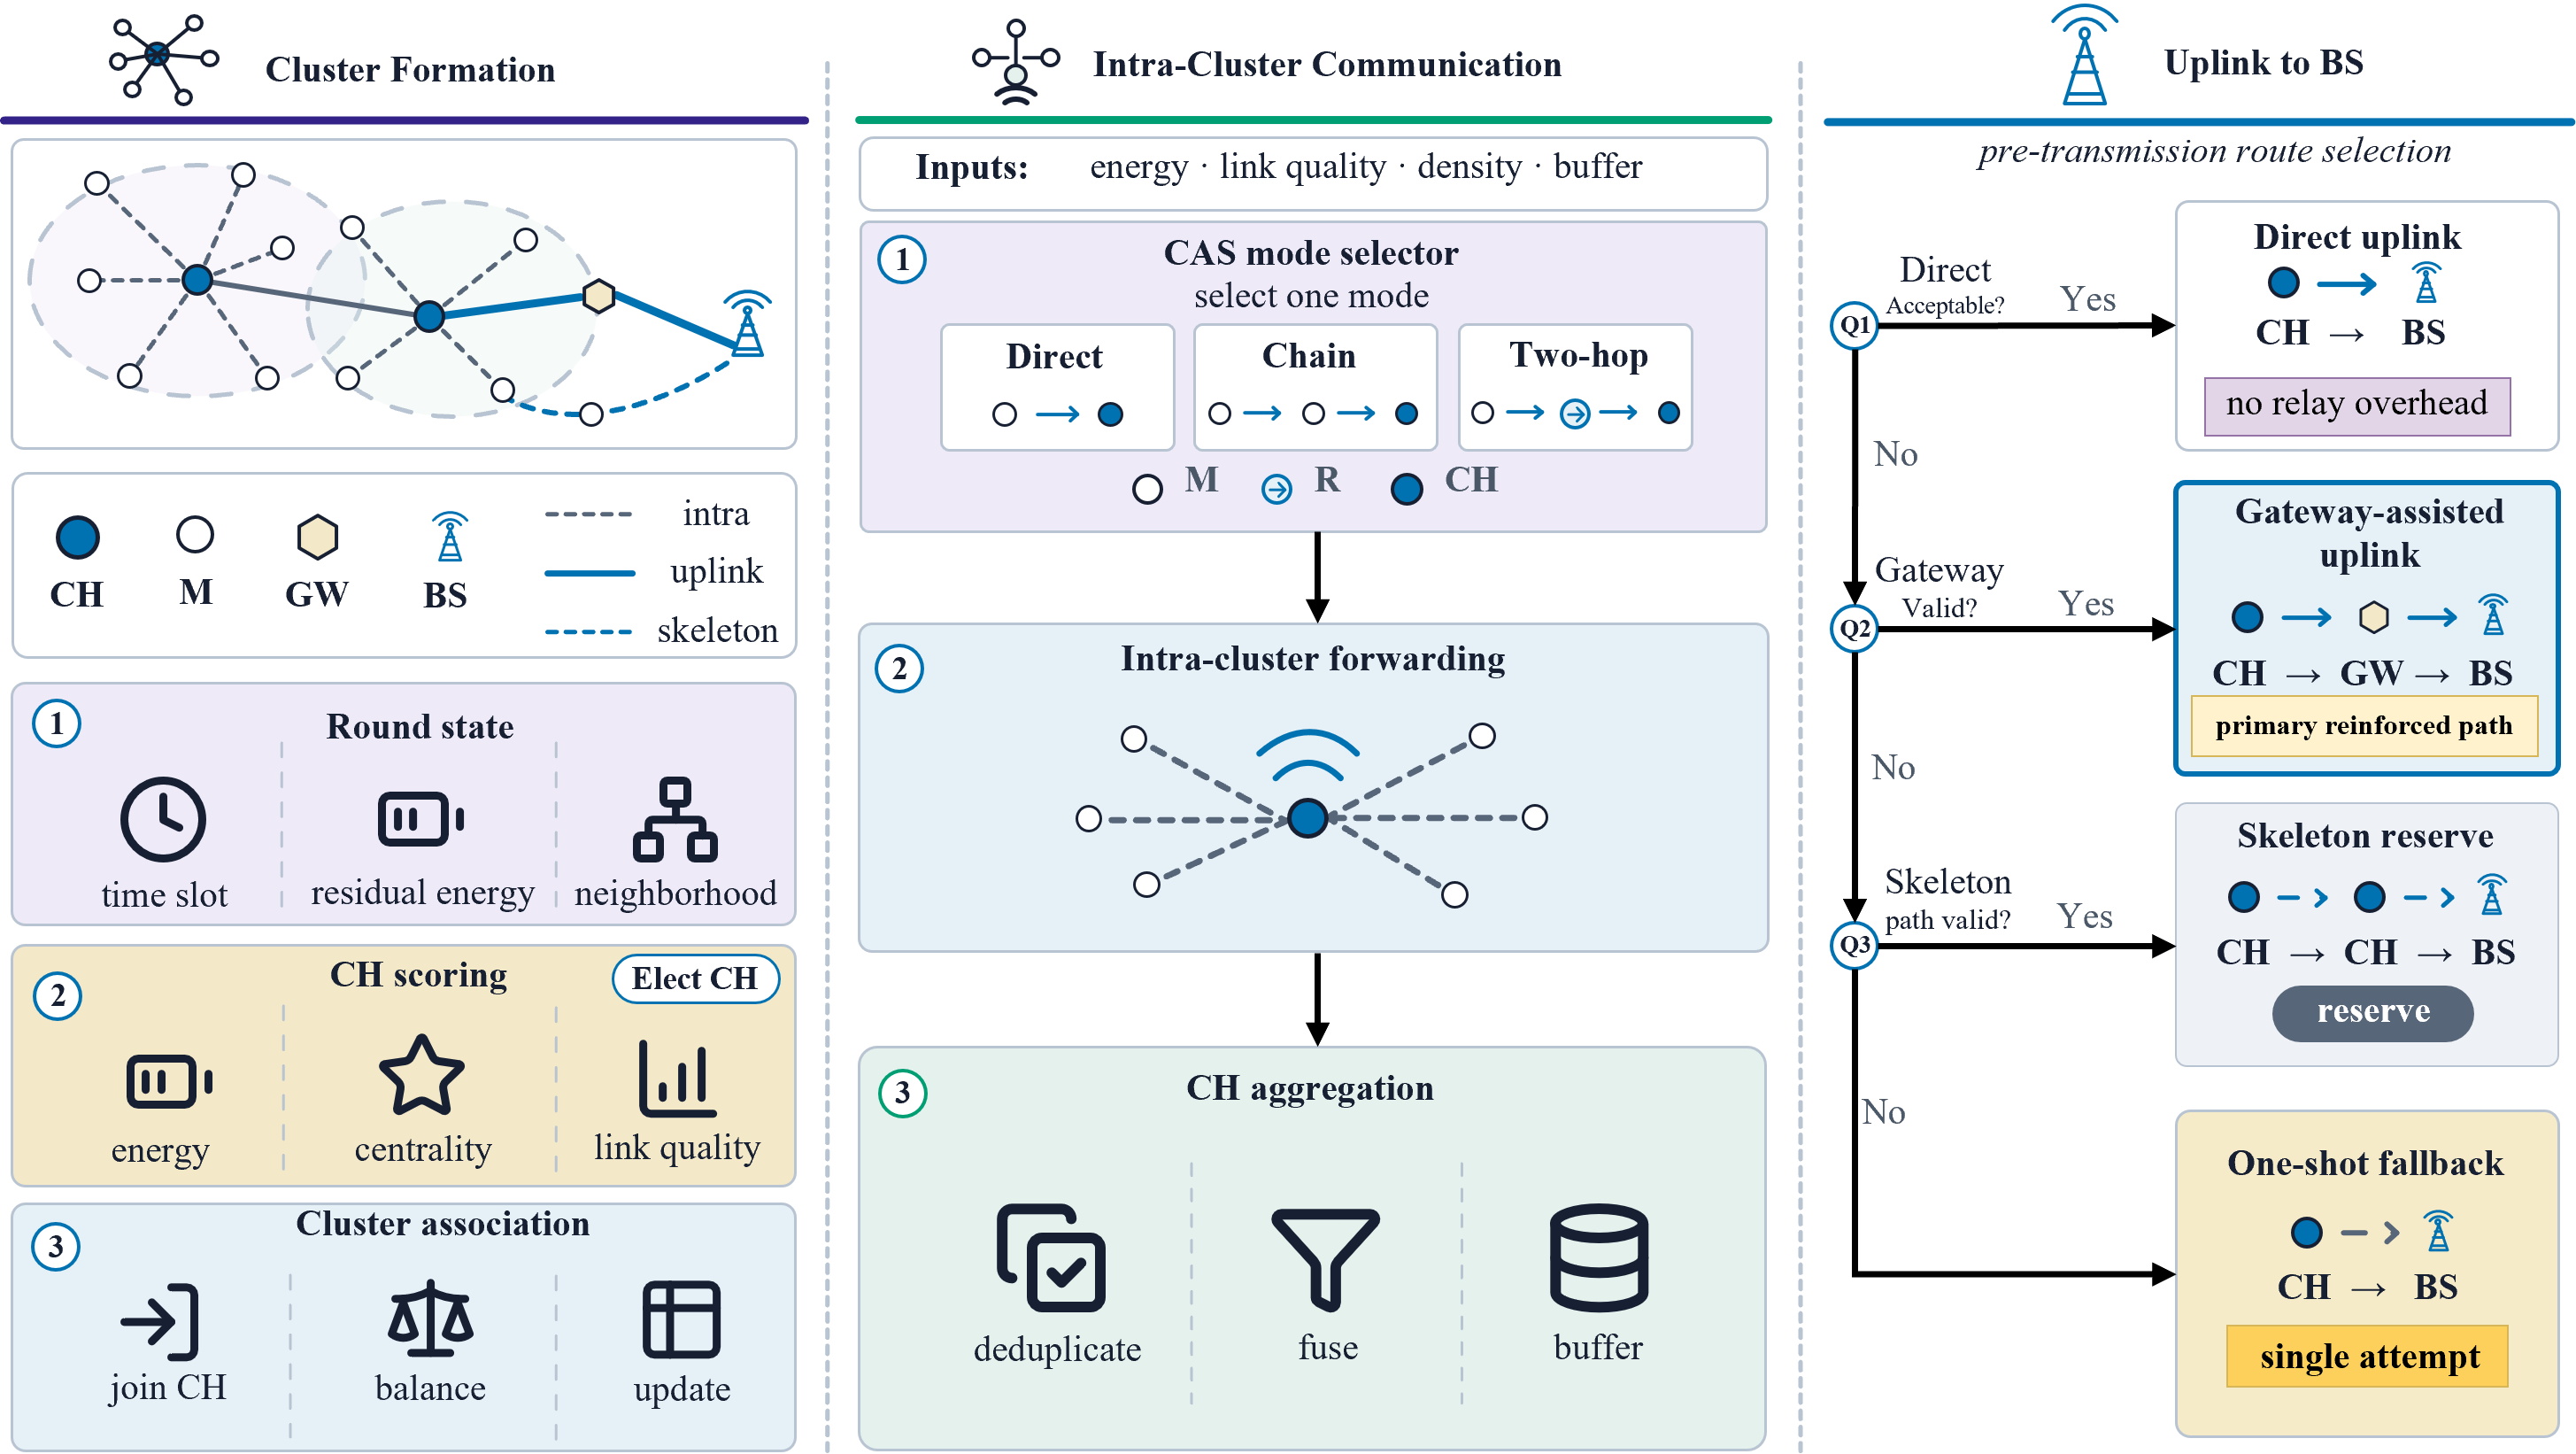
\includegraphics[width=0.92\textwidth]{figures/fig1_workflow.png}
\caption{AERIS round framework. The protocol first forms clusters and scores CH/Gateway candidates, then selects one CAS intra-cluster forwarding mode, and finally applies a first-hit uplink selector over direct, Gateway-assisted, Skeleton-reserve, and one-shot fallback paths.}
\label{fig:aeris_workflow}
\end{figure*}

\section{Related Work}
Classical low-overhead WSN protocols continue to define the primary engineering operating points. LEACH and HEED mitigate long-range transmission costs via clustering, though their uplink quality remains highly sensitive to head placement and channel degradation~\cite{heinzelman2002application,younis2004heed}. PEGASIS distributes load through chain forwarding, but this robustness incurs the cost of increased latency and serialization~\cite{lindsey2002pegasis}. While TEEN suppresses redundant transmissions, its logic makes performance metrics sensitive to the specific definition of ``expected'' delivery~\cite{manjeshwar2001teen}. LCN work has also examined scalable downward routing for WSN and IoT actuation~\cite{zhong2018scalable}. Collectively, these protocols and systems represent the reliability-energy-latency trade-off that any contemporary design must confront.

Recent research has sought to improve reliability through machine learning, hybrid control, and context-aware adaptation~\cite{kumar2019machine,hu2024security,pushpa2025optimizing,tossa2025wireless,wang2024energy,khedr2025advancing,almutairi2025secured}. AERIS aligns with the objective of context-awareness but deliberately maintains a simple runtime logic: it relies on fixed coefficients and explicit control paths without training-time dependencies. Alongside a broader trend toward complex AI-driven routing and sophisticated LLN management documented in recent surveys~\cite{almutairi2024survey,djennadi2025exploring,thakur2025ai}, emerging designs frequently explore reinforcement learning and federated DDQN strategies~\cite{ren2023mefi,okine2024multi,singh2025enhanced,bhukya2025hybrid}.

Collection-tree and RPL-style protocols remain critical because they address the parent-selection problem through structured control planes. CTP constructs trees based on path quality~\cite{gnawali2009collection}, while RPL and MRHOF standardize DAG construction for lossy networks~\cite{tsvetkov2011rpl,gnawali2012minimum}. Opportunistic variants like ORW and ORPL further exploit link diversity~\cite{landsiedel2012low,duquennoy2013let}. This paper does not seek to replace these mature families. Instead, it investigates where a simpler fixed-rule design provides a sufficient reliability gain and where the established collection-tree paradigm should remain the default choice.

\section{Method}
This section introduces AERIS, whose architecture is illustrated in Fig.~\ref{fig:aeris_workflow}. We first define the round-level routing model, then describe the overall forwarding pipeline and its three functional components: cluster formation with context-adaptive intra-cluster forwarding, Gateway-assisted uplink reinforcement, and a sparse Skeleton reserve path. The design objective is not to build a full collection-tree stack. Instead, AERIS provides a deterministic reliability-first controller whose decisions can be traced to local channel, energy, and topology features.

\subsection{Problem Formulation and Round State}
AERIS is a round-based protocol. At the start of each round, every live node exposes a compact local state vector
\begin{equation}
\mathbf{x}_i=[\hat{E}_i,\hat{L}_i,\hat{D}_{iB},\hat{C}_i,\hat{\rho}_i,\hat{U}_i,p_i]^\top .
\end{equation}
Here $\hat{E}_i$ is normalized residual energy, $\hat{L}_i$ is the current link-quality estimate, $\hat{D}_{iB}$ is normalized distance to the base station (BS), $\hat{C}_i$ is a neighborhood-centrality surrogate, $\hat{\rho}_i$ represents local density, $\hat{U}_i$ denotes recent forwarding utilization, and $p_i$ is the historical cluster-head (CH) duty penalty. All variables are normalized to $[0,1]$ before scoring. The protocol does not solve a global optimization problem; instead, it applies fixed scores and deterministic eligibility checks. This choice is intentional: the goal is to expose why a path was selected and to keep the routing behavior reproducible across environments.

A live source generates one sensing report per round. A report is counted as delivered only if it reaches the BS after both the intra-cluster step and the CH-to-BS uplink step succeed. AERIS therefore optimizes complete collection delivery rather than hop-local reception. The routing decision is constrained to local state: nodes do not exchange global topology maps, and CHs do not maintain multi-parent routing tables. This is weaker than a full collection-tree control plane, but it makes each routing transition inspectable.

\subsection{AERIS Framework}
Each round follows five steps. First, live nodes refresh their energy, link, and neighborhood summaries. Second, CHs are elected and ordinary nodes associate with eligible CHs according to local distance, link, and energy features. Third, candidate Gateways and reserve Skeleton nodes are identified from the CH set. Fourth, each cluster selects one intra-cluster forwarding mode through CAS. Fifth, CH traffic is forwarded to the BS through a first-hit uplink selector: direct transmission, Gateway-assisted relay, Skeleton reserve path, and one-shot direct fallback. The selector stops after the first eligible path succeeds, so later fallback paths are not used unless earlier paths are unavailable or fail.

The round abstraction also fixes the information boundary used by AERIS. Nodes do not exchange global topology maps, and CHs do not maintain multi-parent routing tables. The only information used by a forwarding decision is the current local feature vector, the CH set, the candidate Gateway/Skeleton set, and the last-round energy/link summaries. This is weaker than a full collection-tree control plane, but it makes the protocol easier to audit: every transition in Fig.~\ref{fig:aeris_workflow} can be traced to one score or one eligibility check.

The equations in this section are intentionally ordered to mirror that control flow: state acquisition, CH election, member association, Gateway eligibility, Gateway scoring, CAS mode selection, first-hit uplink precedence, delivery accounting, and energy update. The paper is therefore not relying on a large number of equations for their own sake; instead, each equation names one routing decision or accounting rule that the implementation actually executes.

\subsection{Cluster Formation}
CH election uses a normalized suitability score over residual energy, node centrality, neighborhood degree, distance to the BS, and link quality:
\begin{equation}
p_i^{\mathrm{CH}}=\mathcal{F}(\hat{E}_i,\hat{C}_i,\hat{d}_i,\hat{D}_{iB},\hat{L}_i)\,(1-0.25\,p_i),
\end{equation}
where $\mathcal{F}$ is the fuzzy CH score used by the implementation, and $\hat{d}_i$ is the normalized degree surrogate. A fairness penalty reduces repeated CH duty through the factor $1-0.25p_i$, where $p_i$ records prior CH use. This makes CH election energy-aware without turning CH rotation into the dominant objective.

After CH election, non-CH nodes join one CH using a fixed weighted rule over distance, link quality, and residual energy:
\begin{equation}
J_{ij}^{\mathrm{join}}=0.45\,(1-\bar{d}_{ij})+0.40\,\hat{L}_{ij}+0.15\,\hat{E}_j .
\end{equation}
The node then chooses $j^\star=\arg\max_{j\in\mathcal{F}_i}J_{ij}^{\mathrm{join}}$. The exact weights and feasibility threshold are reported with the experimental configuration in Table~\ref{tbl:aeris_params}. If no feasible CH is available, the node attaches to the best available CH and the later uplink selector handles the weak path. This separation keeps local cluster association simple while leaving long-range reliability decisions to the Gateway/Skeleton layer.

\subsection{Gateway-Assisted Uplink}
The Gateway layer targets the fragile CH-to-BS segment. A CH that is close to the BS or already has a reliable uplink sends directly. Otherwise, AERIS searches for a better-positioned CH that can serve as an intermediate relay. Gateway candidates are ranked by a fixed linear score,
\begin{equation}
S_i^{\mathrm{GW}}=w_D\bar{D}_i+w_C\hat{C}_i+w_L\hat{L}_i+w_E\hat{E}_i .
\end{equation}
where $\bar{D}_i$ is normalized CH-to-BS distance, and $\hat{C}_i$, $\hat{L}_i$, and $\hat{E}_i$ are normalized centrality, link quality, and residual energy. The highest-score candidate $g^\star=\arg\max_{g\in\mathcal{G}_k}S_g^{\mathrm{GW}}$ is selected, and the fixed publication weights are reported with the experimental configuration in Section~IV-A.

The selected Gateway aggregates the originating CH's payload with its own CH traffic and forwards the resulting packet toward the BS. If the Gateway uplink fails, AERIS permits a bounded direct rescue from the originating CH. This behavior is deliberately modest: Gateway support is not a full collection tree and does not maintain a long-lived parent structure. It is a local reliability reinforcement mechanism for rounds in which the direct CH-to-BS path is weak.

Gateway activation is controlled by eligibility rather than by a global route recomputation. For a source CH $k$, the candidate set is
\begin{equation}
\mathcal{G}_k=\{g\in\mathcal{H}:E_g>0,\ D_{gB}<D_{kB},\ q_{kg}q_{gB}\ge q_{kB}\},
\end{equation}
where $\mathcal{H}$ is the live CH set and $q_{ab}$ is the estimated one-hop success probability between nodes $a$ and $b$. This filter requires a candidate to be live, geometrically useful relative to the BS, and not weaker than the direct uplink it replaces. Among eligible candidates, the highest fixed score is chosen. If no candidate satisfies the eligibility filter, the CH does not search deeper; it either uses the Skeleton reserve if available or falls back to direct transmission. This shallow decision tree is important for the paper's positioning. It explains why AERIS can be described as auditable, but it also explains why richer CTP/RPL-style baselines can dominate in regimes where repeated parent repair and path-cost updates are beneficial.

\subsection{Context-Adaptive Intra-Cluster Forwarding}
CAS chooses how member traffic reaches the CH before the CH attempts its uplink. It compares direct, chain, and two-hop forwarding using a fixed linear mode score:
\begin{equation}
m_c^{\star}=\arg\max_{m\in\mathcal{M}}\theta_m^\top\phi_c,\quad \mathcal{M}=\{D,C,H_2\}.
\end{equation}
Here $D$, $C$, and $H_2$ denote direct, chain, and two-hop forwarding. The vector $\phi_c$ stacks the cluster-level energy, link quality, BS distance, radius, density, and fairness features. Rule overrides are applied only for obvious reliability cases, such as weak long local links where a short two-hop detour remains available.

The three CAS modes have distinct roles. Direct mode minimizes forwarding overhead when intra-cluster links are already reliable. Chain mode serializes local traffic through short hops in denser clusters, which can reduce weak long local links but may increase latency. Two-hop mode inserts one short relay between a member and its CH, which is most useful when local links are unstable but a nearby relay remains viable. CAS therefore does not claim to be a universally beneficial module; it is an explicit switch that exposes when local detours are selected and when the protocol falls back to simpler forwarding.

\subsection{Skeleton Reserve Path}
The Skeleton layer is a deterministic reserve, not the primary gain carrier. A sparse set of CHs is selected along a principal spatial axis to provide a fallback relay backbone when direct and Gateway paths are not usable. The reserve path is intentionally conservative: it is activated only after earlier uplink choices fail eligibility or delivery, and it does not continuously maintain a dense mesh. This choice limits control overhead but also explains the mechanism results in Section~IV: in the audited configuration, Gateway support resolves most eligible fallback cases, so Skeleton usage remains mostly dormant.

The resulting uplink decision is a first-hit cascade rather than a multipath search:
\begin{equation}
u_k^\star=\begin{cases}
\mathrm{direct}, & \chi_k^{\mathrm{dir}}=1,\\
\mathrm{GW}, & \chi_k^{\mathrm{GW}}=1,\\
\mathrm{Sk}, & \chi_k^{\mathrm{Sk}}=1,\\
\mathrm{fallback}, & \text{otherwise}.
\end{cases}
\end{equation}

\subsection{Failure Handling and State Update}
AERIS treats a forwarding attempt as failed when the selected hop does not deliver under the current channel realization after the configured attempt budget. A direct CH-to-BS success ends the uplink stage. A Gateway success is counted only after both the source-CH-to-Gateway hop and the Gateway-to-BS hop succeed. Skeleton success is counted only if the reserve path reaches the BS. These definitions are used consistently in the NS-3 and stress-layer accounting so that the reported end-to-end PDR measures complete delivery rather than partial hop success.

For source $i$ in round $r$, end-to-end delivery is recorded as
\begin{equation}
d_i^{(r)}=\mathbf{1}\{z_{i,c(i)}^{(r)}=1\}\mathbf{1}\{z_{c(i),B}^{(r)}=1\},
\end{equation}
where $c(i)$ is the assigned CH, $z_{i,c(i)}^{(r)}$ records successful intra-cluster delivery, and $z_{c(i),B}^{(r)}$ records successful CH-to-BS delivery through the selected uplink stage. This definition is strict: a packet that reaches an intermediate relay but not the BS is not counted as delivered.

After each round, residual energy is decremented for transmission and reception events,
\begin{equation}
E_i^{(r+1)}=\max\{0,E_i^{(r)}-\epsilon_{\mathrm{tx}}T_i^{(r)}-\epsilon_{\mathrm{rx}}R_i^{(r)}\},
\end{equation}
where $T_i^{(r)}$ and $R_i^{(r)}$ are the numbers of transmit and receive events charged to node $i$ in round $r$. Link summaries are then refreshed and CH-duty penalties are updated. A node that exhausts its energy is removed from the candidate pool in subsequent rounds. This update rule is the source of the reliability-lifetime trade-off observed later: the Gateway path can protect delivery in harsh cells, but the same relays may accumulate forwarding load and trigger early first-node death. AERIS therefore does not hide relay concentration; it exposes the concentration through the mechanism and lifetime metrics.

\subsection{Packet and Aggregation Semantics}
The protocol is evaluated as a data-collection workload in which each live source is expected to contribute one application reading per round. Member nodes first send readings toward their CH according to the CAS-selected local mode. The CH then aggregates the received readings into the CH payload for that round. A successful end-to-end delivery requires that the aggregated payload reach the BS through one of the uplink paths. This convention matches the intended WSN use case: the routing rule is judged by whether source readings reach the sink, not merely by whether an intermediate relay receives a packet.

Gateway forwarding preserves this accounting. When a source CH uses a Gateway, the source CH's aggregated payload is first delivered to the selected Gateway. The Gateway then forwards a combined uplink payload to the BS. If the source-to-Gateway hop succeeds but the Gateway-to-BS hop fails, the original source readings are not counted as delivered. Likewise, if a member packet fails before reaching its CH, that member reading cannot be recovered by a later CH-to-BS success. This end-to-end accounting is stricter than hop-local success and is why the paper reports PDR over expected application-layer transmissions.

The same semantics also make TEEN comparisons delicate. TEEN is event-triggered and may intentionally suppress transmissions. The evaluation uses a fixed expected denominator so that suppression is not mistaken for reliable delivery. This choice is appropriate for a reliability-first collection workload, but it is not the only possible interpretation of TEEN. A TEEN-centered study should also report event-detection success or actual-transmission PDR. In this paper, TEEN is included to represent a classical threshold-triggered WSN baseline, and its results are interpreted together with energy, lifetime, FND, and hop count.

\subsection{Non-Assumptions}
AERIS does not assume a mobile sink, synchronized channel hopping, time-slotted scheduling, or a standards-compliant 6TiSCH/RPL stack. It also does not assume that every node can hear every CH or that Gateway candidates are always available. If no eligible Gateway exists, the route selector falls through to the next reserve option. If the Skeleton reserve is also not useful, the protocol returns to direct rescue rather than inventing an unmodeled path. These non-assumptions keep the implementation aligned with the evidence: the reported gains come from fixed local routing decisions under the tested channel models, not from hidden full-stack repair behavior.

This also limits the claim. In networks with stable parent sets and enough control budget, a mature collection-tree implementation can outperform AERIS because it maintains richer path information. In deployments where lifetime is the dominant metric, AERIS can be unattractive because Gateway relays concentrate load. The purpose of the method is therefore not to define a universal routing replacement. It is to specify a simple reliability-first controller whose decisions are explicit enough to be audited and whose deployment boundary can be measured.

\subsection{Control Cost}
AERIS keeps per-round control state bounded by local summaries and CH-level relay candidates. Ordinary nodes maintain their own energy/link state and one CH association. CHs maintain member summaries, one CAS mode, and at most one selected Gateway candidate in the publication configuration. The online scoring operations are linear in the number of local candidates: CH election scans live nodes, cluster association scans CHs, Gateway selection scans CH candidates, and CAS compares three fixed mode scores. No training, route-table diffusion, DODAG repair, or global path optimization is performed during the reported runs. The trade-off is that AERIS sacrifices the richer repair behavior of CTP/RPL-style stacks for a smaller and more transparent control path.

Let $N$ be the number of live nodes, $K$ the number of CHs, and $d_i$ the local neighbor count of node $i$. CH election is $O(N)$ after local feature refresh, cluster association is $O(NK)$ in the standalone harness, Gateway ranking is $O(K)$ per source CH, and CAS is $O(1)$ because only three modes are scored. The memory footprint is also local: ordinary nodes keep one association and a small feature vector, while CHs keep member summaries and relay candidates. These bounds are not presented as a theoretical optimality claim; they specify the implementation envelope used in the experiments and clarify why AERIS is simpler than a full collection-tree stack.

\subsection{Decision Precedence}
The most important implementation detail is the precedence among modules. CAS and Gateway do not compete for the same decision. CAS only determines how non-CH nodes deliver data to their CH. Gateway and Skeleton operate after intra-cluster delivery, when the CH must forward aggregated traffic to the BS. This separation prevents a local CAS choice from masking an uplink failure and prevents the Gateway mechanism from changing member-to-CH routing. The resulting behavior is easier to diagnose: if end-to-end delivery falls, the failure can be attributed to intra-cluster delivery, Gateway uplink delivery, Skeleton fallback, or final direct rescue.

The uplink selector is intentionally ordered. Direct transmission is attempted when the CH-to-BS path is eligible, because it adds no relay burden. Gateway transmission is considered next because it is the main reliability reinforcement mechanism and uses only one intermediate CH. Skeleton fallback is later because it can introduce a longer reserve path and is meant to be used sparingly. A final direct rescue is allowed after Gateway failure so that a transient relay failure does not automatically discard a packet that might still be delivered by the source CH. This order is fixed in all reported runs and is not changed per environment.

The same precedence also defines how control overhead is contained. AERIS does not flood route discovery messages after every failure. A failed direct attempt does not trigger a network-wide search; it only advances the local selector to the next eligible option. A failed Gateway attempt does not build a new tree; it permits the configured rescue path and then lets the next round refresh the state. This is one reason the design should be read as a reliability-first WSN controller rather than a full LLN routing stack.

\subsection{Eligibility Rules and Routing Invariants}
The implementation enforces three routing invariants. First, a relay is never selected only because it improves a score; it must also pass an eligibility filter. Direct CH-to-BS forwarding is eligible when the current link estimate is high enough for the configured attempt budget. Gateway forwarding is eligible only if the candidate is live, belongs to the current CH set, is geometrically closer or more useful for the BS direction than the source CH, and has an estimated source-to-Gateway and Gateway-to-BS path that is not weaker than the direct uplink being replaced. Skeleton forwarding is eligible only after the direct and Gateway choices fail eligibility or delivery. These filters prevent the score from selecting a relay that is numerically attractive but topologically useless.

Second, AERIS uses first-hit delivery accounting. Once a packet is delivered by an earlier eligible stage, later stages are not evaluated for that packet. This matters for energy and lifetime accounting because the protocol does not pay for unused fallback paths. It also matters for interpreting the mechanism study: a dormant Skeleton count does not mean the reserve path is absent from the design, but that earlier Gateway decisions already resolved most audited fallback cases.

Third, AERIS keeps routing state round-local. A successful Gateway in one round does not become a persistent parent in the next round, and a failed Gateway does not trigger a long-lived blacklist unless the next feature refresh also lowers its score or eligibility. This design makes AERIS less adaptive than a collection tree, but it avoids hidden history-dependent behavior. The same topology and seed therefore reproduce the same score ordering, fallback order, and delivery accounting, which is important for a protocol whose main claim is auditability rather than learning-based optimality.

\subsection{Relation to Collection-Tree Routing}
AERIS and collection-tree routing both address weak multi-hop delivery, but they do so with different control assumptions, different repair costs, and different state requirements. CTP/RPL-style designs maintain parent/path-cost state and can repair routes through a richer control plane. AERIS does not maintain a DODAG, does not run Trickle-style dissemination, and does not optimize a cumulative path metric. It instead uses one-hop CH-level reinforcement and a sparse reserve path. This makes AERIS weaker than mature collection-tree stacks in some regimes, but it also keeps the decision process compact enough for direct inspection.

This distinction also explains the structure of the evaluation. The classical-baseline audit tests whether AERIS improves over clustering, chain, residual-energy, and threshold-triggered WSN protocols. The expanded boundary sweep then asks whether that improvement remains once simplified collection-style baselines are added. The expected answer is not universal dominance. If CTP/RPL-style parent selection already identifies stable paths in a given cell, AERIS should not be expected to win. The relevant contribution is the deployment boundary: AERIS is useful when a simple fixed controller provides enough uplink reinforcement without the full control machinery of a collection-tree stack.

\section{Experiments}
\subsection{Experimental Setup}
The primary metric is packet delivery ratio over expected application-layer transmissions,
\begin{equation}
\mathrm{PDR}_{\mathrm{expected}}=\frac{N_{\mathrm{delivered}}}{N_{\mathrm{expected}}},
\end{equation}
where $N_{\mathrm{expected}}$ counts one packet per alive source node per round even if a protocol suppresses actual transmission. The denominator is kept fixed across protocols so that the reliability comparison is not confounded by protocol-specific reporting logic.

For Fig.~\ref{fig:classical_margin}, the plotted value is the signed classical margin
\begin{equation}
\Delta_{e,n}=\mathrm{PDR}_{\mathrm{AERIS}}(e,n)-\max_{b\in\mathcal{B}_{\mathrm{classical}}}\mathrm{PDR}_b(e,n),
\end{equation}
where $\mathcal{B}_{\mathrm{classical}}=\{\mathrm{LEACH},\mathrm{PEGASIS},\mathrm{HEED},\mathrm{TEEN}\}$. Positive values mean that AERIS outperforms the strongest classical baseline in the corresponding environment-node cell.

We use four complementary settings. A five-protocol NS-3 comparison evaluates AERIS against LEACH, PEGASIS, HEED, and TEEN across four environments and 100, 500, and 1000 nodes ($n=30$ per cell). An expanded NS-3 boundary sweep adds simplified CTP- and RPL-MRHOF-style collection baselines over 50--1000 nodes. In this standalone harness, CTP and RPL-MRHOF are simplified collection-style baselines rather than complete LLN stacks. Our CTP variant follows the link-cost forwarding rule of \cite{gnawali2009collection} but omits the 4-bit beacon-driven link estimator, dynamic beacon timer, and datapath validation. Our RPL-MRHOF variant follows the path-cost parent selection of \cite{tsvetkov2011rpl,gnawali2012minimum} but omits trickle-driven DIO/DAO, full DODAG repair, and rank-based loop avoidance. These simplifications remove parts of the standards-compliant control plane and repair machinery, so the AERIS--baseline results should be read as a controlled collection-style boundary comparison. Full Contiki-NG/TinyOS stacks may shift the boundary in either direction. Opportunistic variants such as ORW/ORPL \cite{landsiedel2012low,duquennoy2013let} and TSCH-based stacks \cite{duquennoy2015orchestra} are deferred to future work.

The baselines are therefore not used for a single leaderboard claim. LEACH, PEGASIS, HEED, and TEEN define the classical WSN comparison. The CTP- and RPL-MRHOF-style variants define a harder boundary test by introducing stronger parent/path selection. The stress layer is kept separate because the classical protocols are minimally relay-enabled there for multi-hop comparability. This separation prevents the paper from mixing canonical baseline ranking, adapted stress behavior, and mechanism diagnosis.

A 3360-run NS-3 ablation compares full AERIS with no-Gateway, no-CAS, and no-CH-score variants. A collision-aware Python stress layer adds explicit collision and relay contention; LEACH, HEED, and TEEN are minimally relay-enabled there for multi-hop comparability. A separate fixed 100-node publication block reports PDR, consumed energy, lifetime, first-node death, and hop count pooled across the four environments. A 400-replicate-per-cell mechanism study covers 12 cells (four environments at 100, 500, and 1000 nodes) and explains which AERIS mechanisms actually fire.

The NS-3 evidence uses a standalone ns-3.40 validation harness. Nodes are uniformly placed in a 200 m $\times$ 200 m field with the sink at the top-center boundary. Runs use 300 rounds, 512-byte packets, 2.0 J initial energy, 10 dBm transmit power, and seeds 42001--42030. The channel combines log-distance loss, shadowing, fading, receiver sensitivity, and packet-error probability. The path-loss/shadowing pairs are office (2.0, 4.5 dB), factory (2.7, 8.5 dB), suburban (2.8, 7.5 dB), and urban (3.4, 12.0 dB). The harness operates above an idealized contention-free MAC abstraction rather than the full IEEE 802.15.4 stack. The collision-aware Python stress layer adds explicit collision and relay contention on top of this abstraction.

\begin{table}[t]
\caption{NS-3 harness parameters used for the canonical and boundary sweeps.}
\label{tbl:ns3_params}
\centering
\scriptsize
\setlength{\tabcolsep}{2pt}
\begin{tabular*}{\columnwidth}{@{\extracolsep{\fill}}cc@{}}
\toprule
Parameter & Setting \\ 
\midrule
Simulator & standalone ns-3.40 harness \\
Deployment area & 200 m $\times$ 200 m, uniform nodes \\
Sink position & top-center boundary \\
Node scales & 50, 100, 200, 300, 500, 800, 1000 \\
Classical audit scales & 100, 500, 1000 \\
Rounds per run & 300 \\
Replicates & 30 seeds per environment-scale-protocol cell \\
Seed block & 42001--42030 \\
Packet size & 512 bytes \\
Initial energy & 2.0 J per node \\
Transmit power & 10 dBm \\
Environment model & log-distance loss + shadowing + fading \\
Office/factory & $(n,\sigma)=(2.0,4.5)$, $(2.7,8.5)$ dB \\
Suburban/urban & $(n,\sigma)=(2.8,7.5)$, $(3.4,12.0)$ dB \\
MAC abstraction & idealized contention-free canonical layer \\
\bottomrule
\end{tabular*}
\end{table}

All AERIS coefficients are fixed once before evaluation. Table~\ref{tbl:aeris_params} lists the publication configuration; no coefficient is retuned between office, factory, suburban, and urban cells. The ablation disables one component at a time while leaving the remaining settings unchanged, so it measures module contribution under the same protocol configuration rather than a retuned variant.

\begin{table}[t]
\caption{Fixed AERIS configuration used in all reported experiments.}
\label{tbl:aeris_params}
\centering
\scriptsize
\setlength{\tabcolsep}{2pt}
\begin{tabular*}{\columnwidth}{@{\extracolsep{\fill}}cc@{}}
\toprule
Item & Setting \\
\midrule
CH fraction & starts at 0.08; clipped to $[0.05,0.20]$ \\
CH score & fuzzy chance with fallback weights $0.4/0.3/0.2/0.1$ \\
Join score & distance/link/energy = $0.45/0.40/0.15$ \\
Minimum join PRR & 0.20 when a feasible CH exists \\
Gateway score & $w_D/w_C/w_L/w_E=-0.7/0.3/0/0$ \\
Gateway recovery & one relay retry plus one direct rescue \\
Skeleton & sparse PCA-axis reserve fallback \\
CAS smoothing & EMA/confidence = $0.2/0.2$ \\
CAS direct row & $(.35,.65,-.25,-.05,.10,-.05)$ \\
CAS chain row & $(.30,.40,.20,.20,.20,-.05)$ \\
CAS two-hop row & $(.20,.25,.50,.15,.05,-.05)$ \\
\bottomrule
\end{tabular*}
\end{table}

The statistical unit is an environment-scale-protocol cell. Figure~\ref{fig:classical_margin} plots the five-protocol canonical audit as AERIS margin over the strongest classical baseline. This keeps the main classical result readable without line overlap and avoids pretending that the canonical audit is a boundary plot. Against classical WSN protocols alone, AERIS is rank-1 in 21 of 28 environment-node cells and top-2 in all 28, which is enough to justify the claim that it is a reliability-first alternative to the classical baselines.

The expanded seven-protocol audit is summarized in text rather than as a separate figure. Once simplified CTP- and RPL-MRHOF-style baselines are included, AERIS remains strongest mainly in outdoor suburban cells; office and most factory/urban cells are better covered by the collection-tree baselines. We therefore treat the seven-protocol audit as a deployment boundary note, not as a replacement for the classical audit.

The ablation uses the same seed structure and environment-scale grid, but compares full AERIS with one disabled component at a time. Figure~\ref{fig:ablation} reports full-minus-ablated PDR deltas in percentage points; positive values mean that removing the module hurts delivery, while negative values mean that the disabled variant delivered more packets in that cell. Statistical support is computed per environment across the seven node scales after Holm correction. This convention is deliberately conservative: it avoids using the 3360-run count as if every packet or round were an independent statistical sample.

The five-protocol NS-3 comparison anchors the classical-baseline ranking; the seven-protocol audit provides the boundary note; the ablation attributes the gain; and the collision-aware stress layer provides stress evidence rather than a second canonical ranking. Lifetime, FND, hops, and energy expose load concentration. For Fig.~\ref{fig:ablation}, module effects are checked with Welch-type cell tests, Hedges' $g$, and Holm correction. In Fig.~\ref{fig:classical_margin}, winner labels should not be over-read because the plot summarizes mean margins rather than a significance map.

\subsection{Classical Audit and Boundary Note}
\begin{figure}[t]
\centering
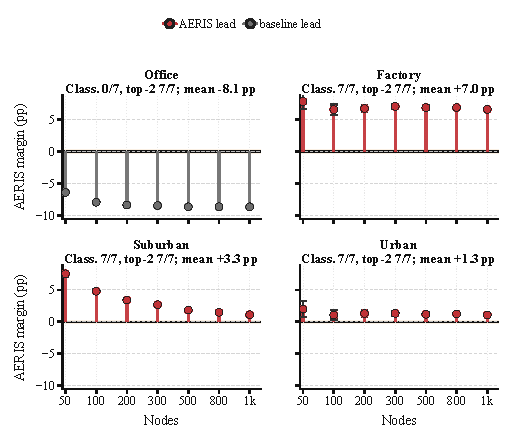
\includegraphics[width=\columnwidth]{figures/fig2_classical_margin.pdf}
\caption{Canonical NS-3 audit across four environments and 50--1000 nodes ($n=30$ per cell). Each marker reports AERIS minus the strongest classical baseline in percentage points; whiskers show approximate 95\% confidence intervals. Red markers favor AERIS, dark gray markers favor the strongest classical baseline, and the light band marks the $\pm$0.1 percentage-point near-tie region. ``Class.'' in each panel title reports AERIS rank-1 coverage against LEACH, PEGASIS, HEED, and TEEN; ``top-2'' reports its top-two coverage in the same classical audit.}
\label{fig:classical_margin}
\end{figure}

Figure~\ref{fig:classical_margin} gives the canonical five-protocol result as signed PDR margins against the strongest classical baseline. This replaces a protocol-line plot because many high-PDR curves overlap visually near the top of the axis; the signed margin exposes the actual classical gain more directly. PEGASIS remains best in indoor office, while AERIS leads in factory, suburban, and urban conditions. The office gap is negative by design, because PEGASIS is the strongest benign-regime baseline in this evidence package. The classical result therefore supports a bounded claim: AERIS is a reliability-first design that remains effective outside the benign office regime.

The seven-protocol audit, which is summarized in text rather than plotted, shows why that claim must still be bounded. Once simplified CTP- and RPL-MRHOF-style baselines are included, AERIS remains strongest mainly in outdoor suburban cells: it wins 6 of 7 scales and is essentially tied at 1000 nodes, where the simplified RPL-MRHOF-style baseline leads by only 0.01 percentage points. In contrast, the RPL-MRHOF-style baseline leads the office cells and most factory and urban cells. AERIS is slightly ahead at factory-50, but falls 1.3--1.8 percentage points behind the RPL-MRHOF-style baseline at larger factory scales; in urban, the average gap to the winner is 5.69 points. AERIS mitigates the fragility of clustering and chain routing by protecting uplinks with Gateway support, but collection-tree and RPL-style baselines already cover part of the same path-selection problem with richer parent choice.

The strongest defensible claim is therefore not that AERIS is globally best, but that its rule-based control path delivers a large gain over classical WSN baselines and remains competitive or best in selected harsh-channel regimes, especially suburban cells.

\subsection{Collision-Aware Stress Evidence}
The five-protocol NS-3 comparison remains the classical-baseline anchor. In that subset, PEGASIS is best in indoor office, while AERIS leads in factory, suburban, and urban conditions. At 1000 nodes, AERIS reaches 0.593 in indoor factory, 0.770 in outdoor suburban, and 0.200 in outdoor urban, compared with 0.324, 0.549, and 0.019 for PEGASIS. The expanded result should therefore be read as a boundary refinement rather than a reversal of the classical-baseline claim.

The collision-aware stress layer asks whether the classical-baseline ordering survives once collision and relay contention are made explicit. Figure~\ref{fig:strict_python} suggests that the ordering is largely preserved under this adapted stress model. PEGASIS remains strongest in indoor office (0.991 at 100 nodes and 0.988 at 1000), whereas AERIS stays rank-1 in indoor factory, outdoor suburban, and outdoor urban. At 1000 nodes, AERIS remains well above PEGASIS in indoor factory (0.728 vs. 0.300) and outdoor suburban (0.728 vs. 0.473), and it still leads in outdoor urban (0.136 vs. 0.099).

Because LEACH, HEED, and TEEN are minimally augmented with a simple relay layer for multi-hop comparability in this setting, Fig.~\ref{fig:strict_python} is stress evidence rather than a second canonical ranking. Its narrower role is to show that AERIS's harsh-channel advantage survives explicit collision-and-relay stress, even though absolute PDR falls for every protocol in the harder scales.

\begin{figure}[t]
\centering
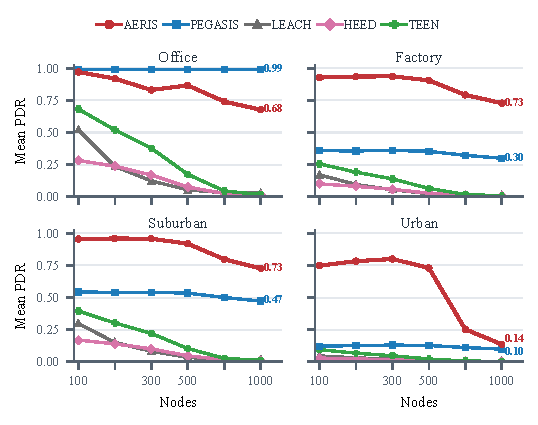
\includegraphics[width=\columnwidth]{figures/fig3_stress.pdf}
\caption{Collision-aware adapted Python stress test across four environments and 100--1000 nodes ($n=3200$ per cell). LEACH, HEED, and TEEN are minimally relay-enabled; this layer tests collision-and-relay stress and is not canonical ranking evidence.}
\label{fig:strict_python}
\end{figure}

\subsection{Ablation}
Figure~\ref{fig:ablation} compresses the full 50--1000 node sweep into a single-column heatmap instead of a wide line plot. Each panel is one disabled module; color encodes full-minus-ablated PDR in percentage points, and filled dots mark Holm-significant cells. This compact view keeps all seven node scales visible without line overlap, but it should be read as a compressed module-effect summary rather than a direct point-by-point trend plot. Gateway is still the main gain carrier in factory and suburban cells across the full grid. Removing Gateway costs 5.82 percentage points on average in factory and 7.58 points in suburban, with all seven node scales significant after Holm correction in both environments. It is essentially neutral in office and weak in urban, which matches the boundary result: office does not need extra uplink protection, while urban links can become too poor for a nearby Gateway to rescue reliably.

\begin{figure}[t]
\centering
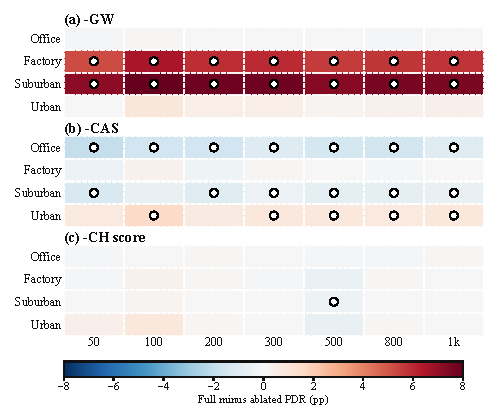
\includegraphics[width=\columnwidth]{figures/fig4_ablation.pdf}
\caption{Compact NS-3 AERIS ablation over the full 50--1000 node sweep ($n=30$ per cell). Each panel is one disabled module. Color encodes full-minus-ablated PDR in percentage points; filled dots mark Holm-corrected significant cells. This single-column heatmap keeps all node scales visible without line overlap.}
\label{fig:ablation}
\end{figure}

CAS has a more mixed role. Removing CAS is beneficial in office and suburban cells, but hurts urban delivery by 0.91 points on average, with five of seven urban scales significant. CAS is therefore not a universal gain module; it is most useful when a short local detour remains viable under harsh links. Removing the CH scoring component is near-neutral in all environments. That does not make the score irrelevant to the design, but it does show that the measured delivery gain in this publication configuration should not be attributed to head scoring.

\subsection{Mechanism and Trade-off}
The 400-replicate-per-cell mechanism study is summarized in Fig.~\ref{fig:mechanism}. It covers 12 environment-scale cells: office, factory, suburban, and urban at 100, 500, and 1000 nodes. Gateway uplink PDR stays near 1.0 in office, factory, and suburban cells, but drops sharply at urban-1000, exactly where end-to-end PDR collapses. A targeted rerun of the three harsh 1000-node cells on an independent machine reproduced the same bottleneck pattern to the reported precision. The visual takeaway matches the ablation: Gateway carries the gain, CAS is conditional, and Skeleton remains dormant because Gateway support resolves most eligible fallback cases in this configuration. These cell-level FND values expose harsh-regime role exhaustion and are not directly comparable to the pooled 100-node block in Table~\ref{tbl:pooled_summary}.

\begin{figure}[t]
\centering
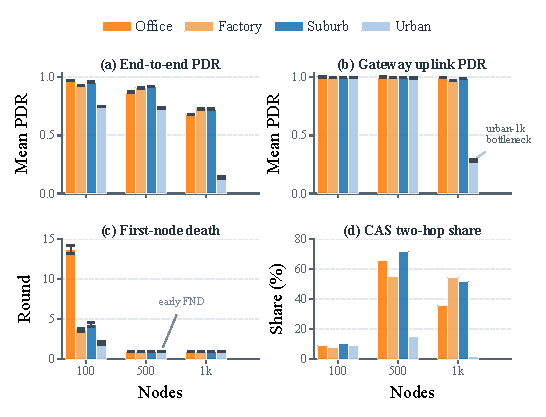
\includegraphics[width=\columnwidth]{figures/fig5_mechanism.pdf}
\caption{AERIS mechanism study from 400 replicates per environment-node cell across 12 cells (4800 runs total). The four panels use grouped bars to show end-to-end PDR, Gateway-uplink PDR, first-node death (FND), and CAS two-hop share by environment and node scale.}
\label{fig:mechanism}
\end{figure}

\begin{table}[t]
\caption{Fixed 100-node pooled trade-off summary.}
\label{tbl:pooled_summary}
\centering
\scriptsize
\setlength{\tabcolsep}{2pt}
\begin{tabular*}{\columnwidth}{@{\extracolsep{\fill}}cccccc@{}}
\toprule
Method & PDR$\uparrow$ & Consumed J$\downarrow$ & Lifetime$\uparrow$ & FND$\uparrow$ & Hops$\downarrow$ \\
\midrule
LEACH & 0.260 & 165.4 & 300.0 & NR & 1.71 \\
HEED & 0.414 & 165.2 & 300.0 & 11.4 & 2.00 \\
TEEN & 0.432 & 159.4 & 299.0 & NR & 1.28 \\
PEGASIS & 0.373 & 137.6 & 300.0 & 70.7 & 32.37 \\
\midrule
\textbf{AERIS} & \textbf{0.674} & \textbf{131.1} & \textbf{215.5} & \textbf{15.8} & \textbf{1.98} \\
\bottomrule
\end{tabular*}
\vspace{1pt}
\parbox{\columnwidth}{\scriptsize\emph{Note:} Values are pooled across the four environments. The broader sweeps in Figs.~\ref{fig:classical_margin}--\ref{fig:ablation} cover 50--1000 nodes. NR = no first-node death before the 300-round horizon. Bold indicates AERIS.}
\end{table}

The trade-off is also clear. Table~\ref{tbl:pooled_summary} shows that AERIS records the lowest consumed energy (131.1 J), but this value reflects early forwarding-role exhaustion rather than an isolated efficiency advantage. It also has the shortest lifetime (215.5 rounds), confirming that delivery is obtained through concentrated relay burden. The PDR improvements quoted in the abstract are computed from the same fixed 100-node block pooled across the four environments. Fig.~\ref{fig:mechanism} localizes the cost to early node death and shrinking two-hop support in harsh cells, but its FND bars are cell-level mechanism measurements rather than the same pooled statistic used in Table~\ref{tbl:pooled_summary}.

Figures~\ref{fig:classical_margin}--\ref{fig:ablation} and Table~\ref{tbl:pooled_summary} suggest a concrete deployment rule. Prefer PEGASIS-like routing when lifetime dominates in benign cells. Consider mature CTP/RPL-style stacks first when richer collection-tree control is acceptable, especially in office, factory, or urban regimes. Choose AERIS when delivery under heterogeneous harsh links is the priority and a simple auditable controller is required, especially in suburban-like cells. Office-like regimes, longevity-first deployments, and mature LLN stacks are the clearest negative cases.

\section{Limitations}
Several limits remain. The expanded seven-protocol audit includes only simplified CTP- and RPL-MRHOF-style collection baselines, not opportunistic routing, ORW/ORPL-style candidate forwarding, coding-based reliability, channel hopping, or standards-compliant Contiki-NG/TinyOS RPL stacks. The AERIS--baseline ordering should therefore be read as a controlled collection-style comparison, not a direct claim against full LLN stacks. The collision-aware stress layer is deployment-stress evidence rather than real-radio-testbed ground truth, and its MAC abstraction omits full 802.15.4/TSCH/CSMA-CA behavior.

Because TEEN is event-triggered, $\mathrm{PDR}_{\mathrm{expected}}$ should be read together with energy, lifetime, FND, and hops; actual-transmission PDR or event-detection success would be needed for a TEEN-centered study. Topology is static, and the environment taxonomy is bounded to the four tested regimes. Recent LLN work likewise emphasizes scalable path management and control-plane flexibility \cite{almutairi2024survey,djennadi2025exploring}. The provenance chain separates native-harness evidence from stress evidence, and a targeted replication of the three harsh 1000-node mechanism cells reproduced the key bottleneck means. All AERIS coefficients and thresholds are fixed once before evaluation; the implementation and raw results will be released publicly upon acceptance.

\section{Conclusion}
This paper evaluates AERIS through a five-protocol NS-3 comparison, a boundary note against stronger collection-tree-style baselines, a collision-aware stress layer, and a mechanism study. The claim is deliberately bounded: AERIS is a reliability-first alternative to classical WSN baselines, but richer collection-tree routing narrows or removes that advantage in office, factory, and urban regimes. Its main contribution is a visible deployment boundary, not a universal ranking. Future work should compare against full RPL/ORW/ORPL-style stacks and more realistic MAC behavior, and test whether Gateway-style reinforcement can coexist with collection-tree parent selection without reproducing the early-node-death cost.

\FloatBarrier
\bibliographystyle{IEEEtran}
\bibliography{ref}

\end{document}
